\chapter{Fundamentação Teórica} 

Com o progresso tecnológico e a crescente importância de monitorar a presença dos alunos, têm surgido sistemas de registro de frequência cada vez mais avançados em várias nações ao redor do globo. No contexto brasileiro, a adoção de tais sistemas também tem se tornando uma prática amplamente adotada nas escolas, buscando assegurar a presença dos alunos e mitigar a taxa de evasão escolar. Através desses sistemas, é possível obter dados precisos sobre a assiduidade dos estudantes, permitindo uma análise mais aprofundada dos padrões de comparecimento e oferecendo informações valiosas para o desenvolvimento de estratégias educacionais eficazes. Além disso, esses sistemas possibilitam um acompanhamento mais individualizado e um monitoramento mais consistente do engajamento dos alunos, contribuindo para a identificação precoce de possíveis problemas e permitindo uma intervenção mais ágil por parte das instituições de ensino. Dessa forma, a utilização de sistemas de frequência representa um importante recurso no esforço contínuo de melhorar a eficiência e a qualidade do sistema educacional brasileiro.

\section{Presença e frequência}

Antes de tratar sobre a análise de dados, é necessário definir a diferença entre as palavras presença e frequência, já que, apesar de semelhantes, os termos não devem ser confundidos pelas etimologias de suas palavras acarretarem significados diferentes. Ou seja, frequência escolar não deve ser confundida com a presença escolar.

A palavra ``frequência'' tem sua origem no latim ``\textit{frequentia}''  \cite{dicionarioëtimologico}, que significa ``ser frequente'' ou ``repetir-se''. O termo ``\textit{frequentia}'' foi incorporado ao latim para expressar a ideia de repetição ou ocorrência frequente de algo. Posteriormente, o termo passou a ser usado na matemática e na física para descrever a quantidade de vezes que um evento se repete em um determinado intervalo de tempo. A partir dessa noção, a palavra ``frequência'' foi adotada em outros contextos, como nas ciências, na linguagem cotidiana e nas tecnologias, para indicar a medida da quantidade, intensidade ou regularidade de algum fenômeno ou evento. Sendo assim,  detecção de frequência em uma sala de aula refere-se à identificação da presença física dos indivíduos naquele espaço. Ela busca determinar se os alunos estão fisicamente presentes na sala de aula, independentemente do nível de participação ou envolvimento. Pode ser realizada por meio de sistemas de monitoramento, como câmeras ou registros de entrada e saída, ou ainda de forma manual, pela anotação de uma pessoa por meio da lista de chamada.

Já a palavra ``presença'' tem sua origem no latim ``\textit{praesentia}'' \cite{dicionarioëtimologico}, que deriva do termo ``\textit{praesens}'', que significa ``presente'' ou "estar ao lado''. ``\textit{Praesens}'' é formado pela junção do prefixo ``\textit{prae-}'', que indica ``antes'' ou ``à frente'', e do verbo ``\textit{esse}'', que significa ``ser'' ou ``estar'' \cite{eti:presenca}. Portanto, a palavra ``presença'' remete à ideia de estar à frente ou ao lado de alguém. Sendo assim, é possível inferir que a detecção de presença em uma sala de aula refere-se não apenas à medição da regularidade com que um aluno participa das atividades educacionais, mas também acompanhar o nível de envolvimento ativo do aluno durante as aulas, a forma com que ele participa, interage com o professor e colegas, realiza tarefas, entre outros aspectos. A detecção de presença busca compreender a consistência com que o estudante se engaja nas atividades ao longo do tempo, podendo ser realizada por meio de sistemas de monitoramento, como câmeras ou sensores de movimento, ou com sensores vestíveis que podem detectar outras informações do estudante, como batimentos cardíacos.

Dessa forma, é possível concluir que a frequência escolar consiste no número de vezes que o aluno frequenta as atividades escolares, enquanto a presença escolar refere-se à participação efetiva do aluno nas atividades escolares. Isso significa que, para ser considerado presente, o aluno precisa não apenas comparecer à escola, mas também participar ativamente das atividades propostas pelos professores, cumprir tarefas, fazer perguntas, entre outras ações que demonstram seu engajamento no processo de aprendizagem. Dessa forma, a presença escolar é considerada um indicador mais abrangente e efetivo do que a frequência escolar, pois leva em conta não apenas a quantidade, mas também a qualidade da participação do aluno nas atividades escolares. Todavia, ainda é importante que a frequência escolar seja acompanhada de perto pelos educadores, juntamente com outros indicadores de desempenho, como as notas e avaliações do aluno, pois, além de ser mais facilmente medida, é ela o critério legal para a manutenção da matrícula escolar \cite{planalto:1996}. Neste trabalho de conclusão de curso, trataremos principalmente da coleta da frequência escolar.

Também é importante destacar que o engajamento e a participação ativa dos alunos nas atividades escolares são fatores determinantes para o sucesso acadêmico. Apenas a presença física na sala de aula não é suficiente para avaliar o envolvimento do aluno com o processo de ensino-aprendizagem, sendo necessário considerar outros indicadores, como a qualidade das tarefas realizadas e a interação com colegas e professores. Nesse sentido, a implementação de sistemas de presença escolar mais sofisticados, capazes de coletar dados precisos sobre a situação do aluno em sala de aula poderia ser uma solução promissora para o aprimoramento das políticas públicas voltadas para a educação \cite{ferreira:2020}.

A compreensão da diferença entre presença e frequência é um aspecto crucial para uma análise precisa dos dados educacionais, sendo fundamental para a compreensão do conceito de pesquisas na área de \textit{Educational Data Mining (EDM)}. Ao entender a diferença entre presença e frequência e o papel do EDM na análise de dados educacionais, é possível explorar como a aplicação desses conceitos e técnicas pode contribuir para aprimorar o sistema educacional, promovendo o engajamento dos estudantes e implementando estratégias eficazes de ensino e aprendizagem.

%%%%%%%%%%%%%%%%%%%%%%%%%%%%%%%%%%%%%%%%%%
%%%%%%%%%%%%%%%%%%%%%%%%%%%%%%%%%%%%%%%%%%

\section{Sistemas de Frequência na Literatura}


\subsection{Iniciativas no exterior}
\label{sec:exterior}

Estudos de ponta sobre sistemas de frequência escolar no exterior costumam ser realizados em países classificados como desenvolvidos, sempre com o objetivo de garantir que os estudantes estejam frequentando as aulas e participando ativamente das atividades escolares, o que contribui para uma educação de qualidade e para a promoção da igualdade de oportunidades na sociedade. Isso pode significar não apenas a detecção da frequência por si só, mas também como o aluno está se comportando dentro da sala de aula, ou seja, se está realmente presente.

Uma das tecnologias mais utilizadas em sistemas de frequência de ponta é a detecção facial, seja por fotos ou por vídeos. Neste contexto, dois trabalhos são apresentados. O primeiro, \cite{bhat:2020}, utilizou a tecnologia de \textit{Deep Learning} para a detecção facial em vídeos de até 33 \textit{frames per second} (fps). O sistema proposto foi desenvolvido com base em uma abordagem de aprendizado de máquina conhecida como \textit{One Shot Learning}, que envolve a capacidade de reconhecer objetos ou rostos com apenas uma única imagem de treinamento, o tornando capaz de identificar um grande número de alunos com apenas uma foto (\textit{frame}) de referência. A precisão do sistema é superior a 90\%, o que faz com que seja possível concluir que o sistema poderia ser útil para aplicação futura não apenas em escolas, mas também em empresas, possuindo baixo custo de implementação.

O segundo trabalho, de \citeonline{chauhan:2022}, implementou um sistema de frequência baseado em reconhecimento facial, utilizando uma metodologia baseada na combinação de Análise de Componentes Principais (PCA) com Redes Neurais Convolucionais (CNN). O sistema é capaz de realizar uma verificação cruzada entre a imagem capturada e as imagens do banco de dados, e registrar a frequência do estudante caso haja correspondência. Os dados são então salvos em uma planilha do \textit{Excel}.

Um outro trabalho apresenta uma maneira de detecção de frequências utilizando Internet das Coisas (IOT). \citeonline{fawaz:2019} teve como objetivo desenvolver um sistema de frequência baseado em \textit{Radio Frequency Identification} (RFID), ou Identificação de Rádio Frequência, com foco em segurança, portabilidade e prontidão para ser implantado em larga escala. O sistema fornece uma solução prática e eficiente para monitorar a frequência dos alunos, utilizando o sistema IoT para registrar e buscar dados em um servidor ou nuvem, tornando-os disponíveis para o usuário a qualquer momento e em qualquer lugar. O trabalho também propõe que os próprios alunos possam conferir os próprios dados a qualquer momento. O artigo de \citeonline{fawaz:2019} também utiliza de um sistema IoT, porém com a tecnologia \textit{Wireless Sensor Networks} (WSNs), cuja proposta era criar cadeiras inteligentes, equipadas com sensores de peso e amplificadores que enviam sinais digitais para um receptor, permitindo a identificação da presença dos alunos durante o horário de aula. Também foi instalado um leitor de impressões digitais para aumentar a segurança e identificação dos alunos.

Outra solução para o problema de detecção de presenças são os dispositivos vestíveis, cujo mapeamento sistemático da literatura de \citeonline{ferreira:2020} aponta bons estudos da área. Segundo os autores, os países que possuem estudos na área são Estados Unidos, França, Itália, China, Japão, Eslovênia e Reino Unido, a maioria com crianças do ensino fundamental de entre 7 a 13 anos. O trabalho investigou o posicionamento dos sensores, a maneira de armazenamento de dados e a validação dos dados, trazendo à tona que alguns dos trabalhos também focavam em coletar dados sobre a saúde física dos estudantes. O trabalho também cita que nenhum estudo brasileiro foi encontrado, trazendo a hipótese de que a baixa qualidade da infraestrutura de muitos contextos educacionais brasileiros poderia ser um impeditivo desse tipo de estudo em território nacional. 

\subsection{Iniciativas no Brasil}
\label{sec:brasil}

A Base de Dados do Cadastro Único para Programas Sociais (CadUnico) é uma ferramenta utilizada pelo Governo Brasileiro para registrar informações sobre famílias em situação de vulnerabilidade social, além de ser uma importante fonte de dados sobre a escolaridade no Brasil, pois registra informações sobre a escolaridade dos membros das famílias cadastradas que são utilizadas para monitorar e avaliar as políticas públicas de educação, bem como para identificar as famílias que precisam de apoio para garantir o acesso e a permanência na escola \cite{garcia:2017}. Desde sua criação, a base de dados CadUnico tem recebido diversos prêmios, como o prêmio de Inovação na Gestão Pública Federal, concedido em 2017 pelo Ministério do Planejamento, Desenvolvimento e Gestão, e o Prêmio Excelência em Governo Eletrônico, concedido em 2016 pela Associação Brasileira de Entidades Estaduais de Tecnologia da Informação e Comunicação.

No que diz respeito à unificação da base de frequência com o chamado Sistema Presença, o Brasil tem buscado implementar medidas para garantir o registro da frequência escolar de todos os estudantes. O Sistema Presença foi lançado em 2019 pelo MEC com o objetivo de padronizar as informações sobre a frequência escolar em todo o país. Antes da criação do sistema, as informações sobre a frequência dos estudantes eram registradas em diferentes sistemas pelos estados e municípios, o que dificultava o acompanhamento e a análise dessas informações. Vale destacar que a chave única de identificação dos alunos neste sistema é o Número de Identificação Social (NIS), que é gerado pelo CadUnico. No entanto, a implementação do Sistema Presença tem enfrentado alguns desafios, como a necessidade de capacitação dos profissionais envolvidos no registro e análise dos dados, para que os responsáveis pela coleta e análise dessas informações estejam devidamente preparados para lidar com as novas tecnologias e sistemas de informação. Outro desafio é a questão de investimentos em infraestrutura tecnológica para garantir o funcionamento do sistema em todo o país, o que envolve desde a aquisição e manutenção de equipamentos e softwares até a disponibilidade de uma conexão de internet estável e rápida, especialmente em regiões mais remotas~\cite{echazarra2019learning}. Por fim, a pandemia de COVID-19 trouxe novos desafios para a implementação do sistema, especialmente no que diz respeito à adaptação do sistema às novas modalidades de ensino remoto. Com a suspensão das aulas presenciais em muitas regiões do país, foi necessário buscar alternativas para registrar a frequência dos estudantes em aulas virtuais e atividades remotas. Isso exigiu uma adaptação rápida do sistema e dos profissionais envolvidos, bem como investimentos adicionais em tecnologias e recursos para permitir a coleta dessas informações.

Com o Sistema Presença, o acompanhamento da frequência dos estudantes tornou-se mais efetivo, mesmo com os desafios de questões profissionais e monetárias, o que pode contribuir para a promoção de políticas públicas mais eficazes na área da educação. Em uma pesquisa realizada pelo MEC, em 2019, ano de implementação do sistema, a frequência escolar alcançou os melhores índices históricos, como é possível verificar pela Figura \ref{fig:my_label} \cite{historicos2019}. As duas imagens representam o histórico de frequência entre os anos de 2007 (um ano após a implementação do Sistema Presença) e 2019, indicando que houve índices recordes de frequência escolar em todo o país; ou seja, a taxa de alunos beneficiários dentro da sala de aula, entre fevereiro e março de 2019, chegou a 90,31\%, e entre abril e maio, em 89,81\%.

\begin{figure}[ht!]
    \centering
    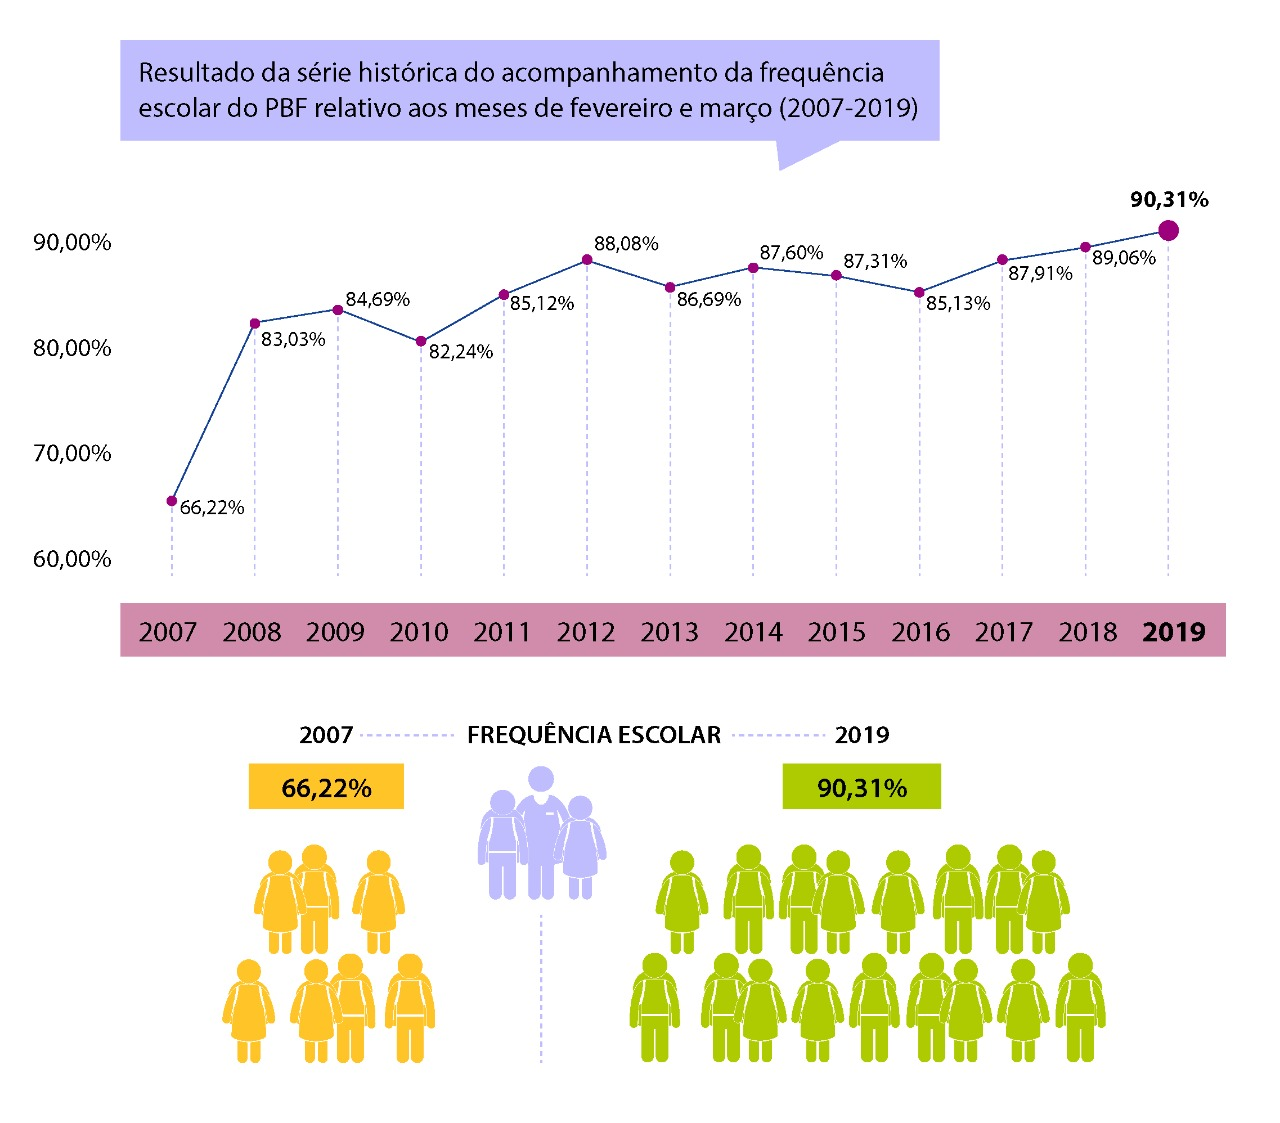
\includegraphics[width=0.46\linewidth]{Textuais/Imagens/image1.png}
    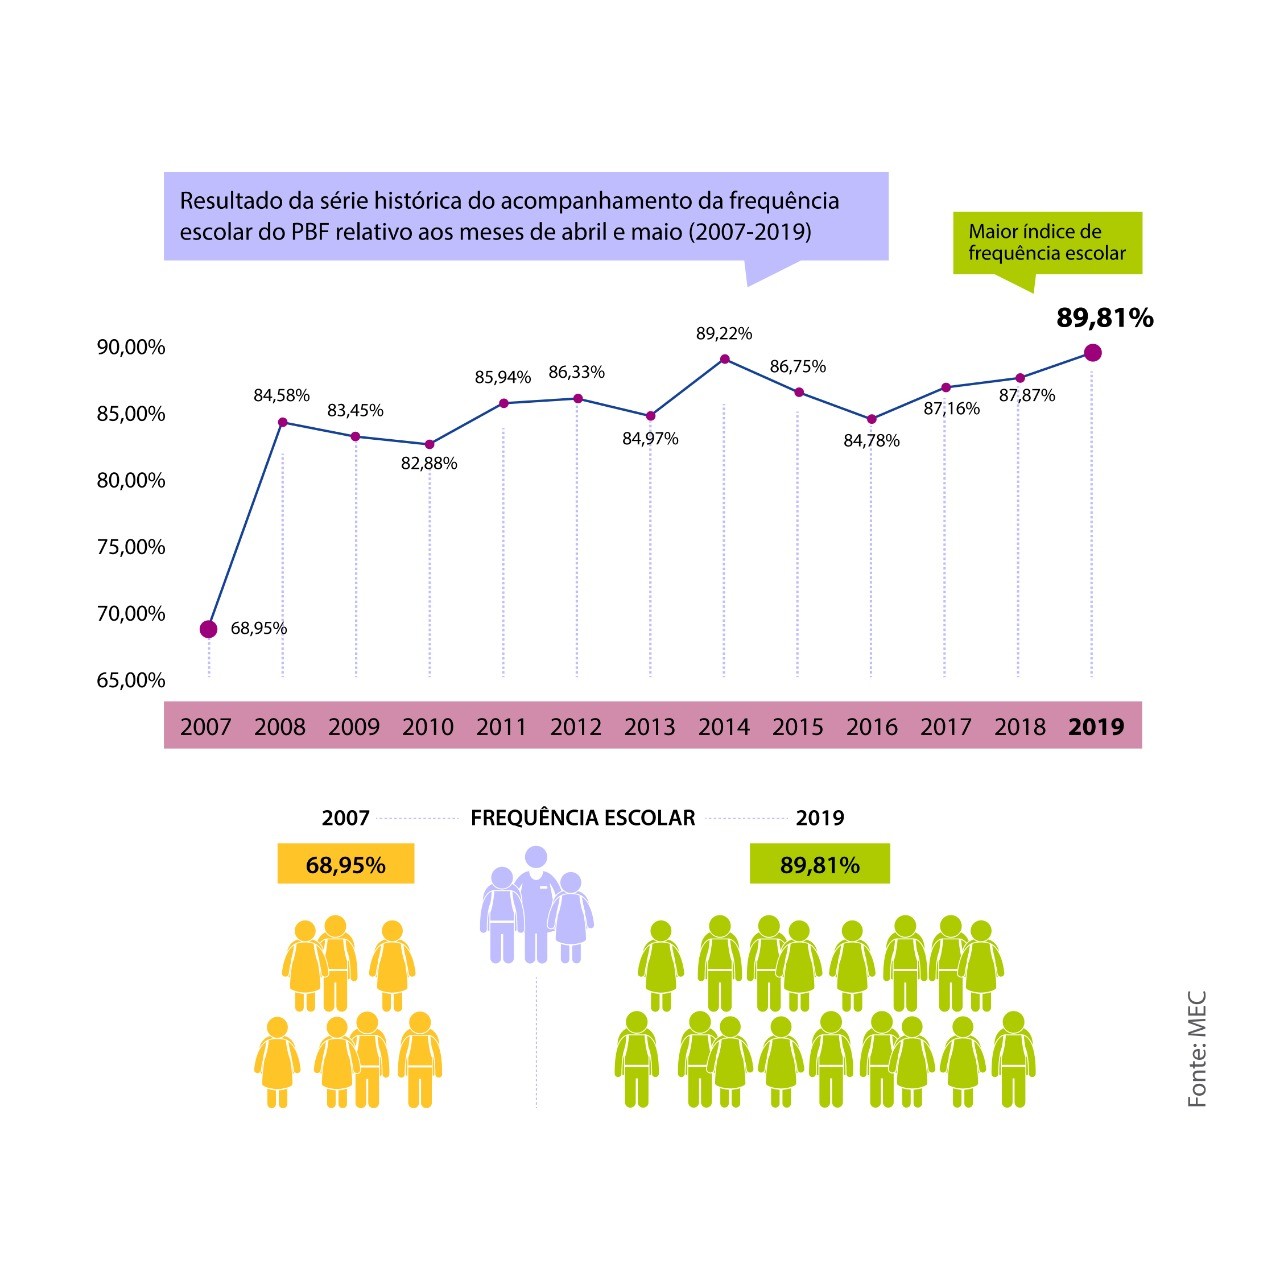
\includegraphics[width=0.46\linewidth]{Textuais/Imagens/image.png}
    \caption{Histórico de frequência de estudantes no Brasil entre os meses de fevereiro e março, e de abril e maio de 2019.}
    \label{fig:my_label}
\end{figure}


O Sistema Presença tem limitações importantes. Como o objetivo deste sistema é fornecer dados para o Bolsa Família, apenas alunos beneficiários deste programa têm sua frequência coletada. Além disso, a frequência é coletada com granularidade mensal. Isto impossibilita o desenvolvimento de ferramentas de alerta de evasão, baseadas em Inteligência Artificial, que sejam capazes de detectar padrões nos dados e permitam ações de combate à evasão em um estágio precoce. Por outro lado, não há a integração dos dados de frequência com outros dados relevantes do estudante, como dados de desempenho escolar. Embora o Sistema Presença ainda esteja em fase de implementação, desde o início dos anos 2000 houveram estudos foram conduzidos com o objetivo de resolver o problema de coleta de dados de frequência de forma mais eficiente \cite{Soligo_2010}. É o caso do trabalho de \citeonline{pereira:2012}, que apresenta uma proposta de monitoramento do estudante no momento de chegada e saída da instituição, sendo realizada em tempo real a comunicação aos responsáveis através do envio de SMS. Adicionalmente, será possível a geração de relatórios acerca da frequência escolar do aluno. A utilização da aplicação proposta visa tornar o controle de frequência mais rápido e eficiente, além de proporcionar a comunicação dos dados coletados aos responsáveis do discente, estabelecendo a sensação de segurança por parte da instituição. Além da frequência, há dispositivos que buscam coletar outros tipos de dados de alunos em sala de aula, como demonstrado no projeto de \citeonline{ferreira:2022}. Neste projeto, foram utilizados objetos vestíveis para detectar os movimentos das crianças do ensino fundamental, a fim de observar o comportamento dos alunos em sala de aula e compreender melhor a rotina escolar. A metodologia utilizada para coletar os dados de movimento das crianças foi a utilização de um dispositivo \textit{wearable Actigraph GT9X Link}, que possui dois acelerômetros e um giroscópio, sendo estes os sensores de captação de movimento. As informações geradas tratam-se de registros em arquivo dos pontos dos eixos de (x, y, z) de cada um dos sensores para cada centésimo de segundo. Para ser traçado o perfil dos estudantes voluntários, foram enviados formulários aos responsáveis que envolviam perguntas como idade, peso, altura, sexo, mão com a qual escreve e se o aluno possui alguma deficiência diagnosticada. Durante a coleta de dados, foram feitas anotações específicas de todos os movimentos, atividades e atenção de cada aluno por um período de 30 minutos, e os demais movimentos no restante do tempo foram anotados apenas quando tratavam-se de levantar, sentar, andar e sair da sala. Por mais que o estudo não fosse conclusivo e não apresentasse resultados específicos da coleta de dados de movimento das crianças, foi concluído que a utilização de sensores vestíveis em sala de aula pode auxiliar o professor a melhorar a qualidade das palestras, especialmente se as informações forem fornecidas em tempo real, principalmente quando os sensores conseguem estimar o nível de engajamento dos alunos na aula e fornecem essa informação diretamente ao educador.

Contudo, é importante reforçar que a coleta de dados educacionais no Brasil apresenta desafios que vão além da infraestrutura de tecnologia da informação. Em regiões mais remotas do país, como comunidades ribeirinhas e áreas rurais, muitas escolas têm dificuldades para enviar e receber informações por meio de sistemas eletrônicos \cite{Ribeirinhas:2021}. Além disso, a realidade das escolas que atendem adolescentes em conflito com a lei, como a Fundação Casa (antiga Febem), também apresenta dificuldades para a coleta de dados educacionais: Em primeiro lugar, muitos desses jovens chegam à instituição com histórico de evasão escolar e baixa escolaridade, o que dificulta o acompanhamento de sua trajetória educacional. A rotatividade de professores e funcionários nessas instituições, aliada a uma infraestrutura muitas vezes precária, pode dificultar o registro e a organização dos dados educacionais dos alunos. Por fim, há ainda a questão da própria natureza das atividades desenvolvidas nessas instituições, que podem ser muito diferentes das atividades escolares convencionais e, portanto, requerem uma avaliação mais específica e adaptada. O atendimento educacional dessas instituições muitas vezes é feito de forma precária e com poucos recursos, o que pode prejudicar a coleta de informações precisas sobre a frequência e o desempenho dos estudantes \cite{Morais2019}. Essas diferenças no contexto educacional brasileiro tornam ainda mais desafiadora a tarefa de coletar e analisar dados educacionais para subsidiar políticas públicas efetivas.

Em suma, a pluralidade brasileira apresenta desafios significativos para a coleta e análise de dados educacionais. Embora iniciativas como o Cadastro Único para Programas Sociais e o Sistema Presença tenham sido criadas para padronizar as informações sobre a frequência escolar e a vulnerabilidade social das famílias, ainda existem muitos obstáculos a serem superados. A infraestrutura de tecnologia da informação, por exemplo, é um desafio em regiões remotas, e a rotatividade de professores e funcionários em instituições como a Fundação Casa pode dificultar o registro e a organização dos dados educacionais dos alunos. Portanto, novas pesquisas podem ser realizadas para aprimorar essas iniciativas e desenvolver soluções tecnológicas que possam superar esses desafios e garantir a coleta de informações precisas sobre a educação no Brasil. Também é importante ressaltar que a avaliação das atividades educacionais em instituições específicas, como a Fundação Casa, requer uma abordagem mais específica e adaptada, uma vez que essas atividades podem ser muito diferentes das atividades escolares convencionais.




%%%%%%%%%%%%%%%%%%%%%%%%%%%%%%%%%%%%%%%%%%
%%%%%%%%%%%%%%%%%%%%%%%%%%%%%%%%%%%%%%%%%%



% Falar sobre o trabalho e explicar sobre o projeto ao qual o trabalho está vinculado.
% Trabalho bem grande que não está desenvolvido por inteiro
% - MEC e NEES
% - objetivo geral é tal
% - x anos
% - existem várias equipes de desenvolvimento, entrando como assistente de pesquisa

%%%%%%%%%%
  
\section{Educational Data Mining (EDM)}

\textit{Data Mining} (DM), ou mineração de dados, é um processo que envolve a descoberta de informações a partir de conjuntos de dados grandes e complexos. Seus conceitos combinam técnicas estatísticas, de banco de dados e de inteligência artificial para explorar os dados e identificar padrões, tendências e relacionamentos ocultos. A mineração de dados permite extrair conhecimentos úteis e significativos a partir de grandes volumes de dados, que podem ser provenientes de diferentes fontes, como bancos de dados corporativos, registros de transações, mídias sociais, registros de compras e muito mais. O objetivo é descobrir padrões consistentes e informações relevantes que possam ser utilizadas para tomar decisões estratégicas, identificar oportunidades de negócio, prever comportamentos futuros e melhorar a eficiência operacional.

O processo de mineração de dados envolve várias etapas, como a coleta de dados de diferentes fontes, o armazenamento em um banco de dados, o pré-processamento dos dados para garantir sua qualidade e consistência, a aplicação de técnicas de mineração de dados para descobrir padrões e relacionamentos, e a interpretação dos resultados obtidos. A mineração de dados desempenha um papel crucial em diversas áreas, tais como marketing, finanças, saúde, varejo, segurança, entre outras. Ela permite identificar segmentos de clientes, prever demandas futuras, otimizar processos, detectar fraudes, personalizar recomendações, melhorar a qualidade do atendimento ao cliente, entre muitas outras aplicações.

A \textit{Educational Data Mining}, ou mineração de dados educacionais, é uma disciplina emergente que é preocupada com o desenvolvimento de métodos para explorar os dados únicos e cada vez mais em grande escala que vêm de ambientes educacionais e usar esses métodos para entender melhor os alunos e os ambientes em que eles aprendem \cite{Egitim:2017}. Sendo assim, EDM é uma área de pesquisa interdisciplinar que combina técnicas de mineração de dados, aprendizado de máquina e estatística para analisar grandes conjuntos de dados educacionais. Seu principal objetivo é analisar dados educacionais para resolver problemas da pesquisa educacional, descobrindo padrões, tendências e relações nos dados coletados a fim de obter conclusões valiosas para melhorar a eficácia do ensino e da aprendizagem.

Através da aplicação de técnicas de mineração de dados e análise estatística, o EDM permite extrair conhecimento a partir de dados educacionais, que podem incluir registros acadêmicos, históricos de notas, interações do aluno com sistemas de aprendizagem online, dados de questionários, entre outros. Esses dados são processados e analisados para identificar padrões e relações que possam ajudar a compreender o desempenho dos alunos, suas dificuldades, preferências de aprendizagem e outros aspectos relevantes.

Alguns exemplos de aplicações do EDM incluem, mas não estão limitados a:

\begin{enumerate}
    \item Previsão do desempenho dos alunos: Ao analisar dados de sistemas educacionais, como informações dos alunos e notas, além de dados de sistemas que não estão diretamente ligados a uma universidade ou escola, como dados de vestibular do Sistema de Seleção Unificada (Sisu) ou Exame Nacional do Ensino Médio (Enem), os pesquisadores podem identificar padrões associados ao sucesso ou fracasso dos estudantes, é possível processar esses dados e identificar padrões e correlações que podem ser usados para prever o desempenho do estudantes \cite{avaandparpinelli:2020}. A previsão do desempenho dos alunos pode trazer diversos benefícios para as instituições de ensino, como a possibilidade de oferecer uma educação personalizada aos alunos de risco e o oferecimento de bolsas para alunos que se destacam.

    \item Identificação de alunos em situação de risco: Ao analisar dados sobre o comportamento e desempenho dos estudantes, os pesquisadores podem identificar fatores associados a resultados acadêmicos insatisfatórios. Por exemplo, eles podem descobrir que os alunos que faltam às aulas ou não concluem as tarefas no prazo têm maior probabilidade de abandonar a escola. Essas informações podem ser utilizadas para desenvolver sistemas de alerta precoce que informam os educadores quando um aluno está em risco de abandonar os estudos, permitindo que intervenham antes que seja tarde demais \cite{ramos:2020}.

    \item Acompanhar automaticamente atividades de estudantes: Ao analisar dados de registro provenientes de plataformas Learning Management Systems (LMS), os pesquisadores podem obter percepções sobre como os estudantes interagem com os materiais do curso e identificar áreas em que possam estar enfrentando dificuldades. Essas informações podem ser utilizadas para personalizar os ambientes de aprendizagem, fornecendo \textit{feedback} direcionado ou recomendações de recursos adicionais \cite{Santos2019}.

    \item Recomendar recursos de aprendizagem aos alunos com base em seu desempenho e preferências: Ao analisar dados sobre o comportamento e desempenho dos estudantes, os pesquisadores podem desenvolver algoritmos que recomendam recursos de aprendizagem específicos de acordo com as necessidades e interesses individuais de cada aluno \cite{9637207}.
\end{enumerate}

Contudo, para se realizar essas pesquisas deve-se coletar e analisar dados de estudantes que podem ser classificados como sensíveis, e portanto há importantes preocupações quanto à privacidade e segurança dos dados, uma vez que a pesquisa, caso feita sem cuidado, pode potencialmente colocar em risco informações pessoais dos estudantes. Além disso, a necessidade de habilidades especializadas para analisar grandes conjuntos de dados pode criar uma barreira para alguns educadores ou instituições que não tenham recursos ou conhecimentos especializados para usar efetivamente essa tecnologia. Outra possível desvantagem é a possibilidade de reforçar vieses existentes nos dados, o que pode perpetuar preconceitos e desigualdades ou limitar oportunidades para determinados grupos de estudantes.


%%%%%%%%%%%%%%%%%%%%%%%%%%%%%%%%%%%%%%%%%%

\subsection{Learning Analytics (LA)}

\textit{Learning Analytics}, ou {analíticas de aprendizado}, é uma área de estudo que utiliza técnicas e ferramentas analíticas para coletar, analisar e interpretar dados relacionados ao processo de aprendizagem. Envolve a aplicação de métodos quantitativos e qualitativos para obter informações útil sobre o desempenho dos estudantes, padrões de comportamento, eficácia do ensino, entre outros aspectos relacionados ao aprendizado. O objetivo principal do \textit{Learning Analytics} é melhorar a eficácia e a eficiência do processo de aprendizagem. Ao coletar dados relevantes, como desempenho acadêmico, interações em plataformas de aprendizado online, tempo gasto em atividades, feedback dos alunos, entre outros, as instituições educacionais podem identificar padrões e tendências que ajudam a entender melhor o progresso dos alunos e oferecer suporte personalizado. As técnicas de \textit{Learning Analytics} podem ser aplicadas em diversos contextos educacionais, desde escolas e universidades até plataformas de ensino online. Com base nas informações coletadas, é possível tomar decisões informadas para aprimorar o planejamento curricular, desenvolver intervenções pedagógicas, identificar necessidades de alunos em risco, personalizar a experiência de aprendizagem e avaliar a eficácia de métodos de ensino específicos.

{Segundo \citeonline{Aldowah2019}, há determinadas etapas necessárias para se conduzir um estudo de Learning Analytics (LA), as quais incluem:}

\begin{enumerate}
    \item {Definir o problema de pesquisa: O primeiro passo é identificar o problema de pesquisa que se deseja abordar. Isso pode envolver a identificação de uma questão específica relacionada ao ensino e aprendizagem que possa ser respondida por meio da análise de dados.}
    \item {Coletar dados: O próximo passo é coletar os dados necessários para responder à questão de pesquisa. Isso pode envolver a coleta de dados de várias fontes, como LMS, registros acadêmicos, questionários de alunos e outros dados relevantes.}
    \item {Pré-processar os dados: Depois que os dados são coletados, eles precisam ser pré-processados para garantir que estejam limpos e prontos para análise. Isso pode envolver a limpeza de dados ausentes ou inconsistentes, a normalização de dados e a seleção de recursos relevantes.}
    \item {Analisar os dados: O próximo passo é analisar os dados usando técnicas de aprendizado de máquina, mineração de dados e outras técnicas de análise de dados. Isso pode envolver a identificação de padrões e tendências nos dados, a criação de modelos preditivos e a realização de outras análises relevantes.}
    \item {Interpretar os resultados: Depois que os dados são analisados, os resultados precisam ser interpretados para responder à questão de pesquisa original. Isso pode envolver a identificação de relevância, a validação dos resultados e a comunicação dos resultados para as partes interessadas relevantes.}
    \item {Tomar medidas: Com base nos resultados da análise, as partes interessadas podem tomar medidas para melhorar o ensino e a aprendizagem. Isso pode envolver a implementação de intervenções específicas para alunos ou grupos de alunos, a revisão de materiais de ensino ou a melhoria de práticas de ensino.}
    
\end{enumerate}

{É notável que no processo de \textit{Learning Analytics} há grande envolvimento da coleta de dados de diversas fontes, como sistemas de gerenciamento de aprendizagem, registros de atividades dos alunos, interações em fóruns e redes sociais, entre outros. Esses dados são então analisados para identificar padrões e tendências que possam ajudar a entender melhor o comportamento dos alunos e o desempenho do sistema educacional como um todo. Uma das principais características de \textit{Learning Analytics} é a sua abordagem holística, que considera o sistema educacional como um todo. Isso significa que a análise de dados não se limita apenas ao desempenho dos alunos, mas também leva em conta fatores como o ambiente de aprendizagem, a qualidade do conteúdo, a eficácia dos métodos de ensino, entre outros.}

{Outra característica importante é a ênfase na intervenção e participação humana. Embora a análise de dados seja realizada por meio de ferramentas computacionais, a interpretação dos resultados e a tomada de decisões são feitas por professores, gestores e outros profissionais da educação \cite{Barone_2020}. Isso significa que a tecnologia é usada como uma ferramenta para apoiar a tomada de decisões, e não como um substituto para o julgamento humano. Isso é uma consideração importante pois os alunos estão em constante mudança de perfil, o que exige novas e eficazes ferramentas para auxiliar nesse processo. Sendo assim, as instituições de ensino vêm produzindo e armazenando grande quantidade de dados ao longo do tempo.}


%%%%%%%%%%%%%%%%%%%%%%%%%%%%%%%%%%%%%%%%%%

\subsection{Conexão entre EDM e LA}

Como visto nas seções anteriores, tanto LA quanto EDM são áreas específicas que são usadas para representar o uso e a aplicação de mineração de dados em diversos contextos educacionais. Elas estabelecem um ecossistema que pode consecutivamente coletar, processar, reportar e trabalhar com dados continuamente para melhorar o processo educacional. Contudo, as etapas de ambos os processos são diferentes.

{Ambas as áreas têm como objetivo a melhoria de processos de ensino e aprendizagem por meio da análise de dados em larga escala, de maneira sistematizada, que possam auxiliar na ampliação de processos de avaliação, compreensão de problemas e planejamento de intervenções. Segundo \citeonline{Moissa2015}, tanto quanto EDM e LA têm como objetivo analisar dados educacionais para entender o processo de ensino e aprendizagem e melhorá-lo, incluindo o uso de algoritmos de aprendizado de máquina, a análise de dados em tempo real e a aplicação de técnicas de análise de redes sociais. Seus resultados e análises podem ser aplicados no desenvolvimento de sistemas de recomendação personalizados para estudantes e professores.}

Uma das principais vantagens em se beneficiar de ambas as áreas é que isso permite aos tomadores de decisão avaliar os processos de aprendizagem dos estudantes e atender às suas diferentes necessidades de aprendizagem com base em seus comportamentos e preferências reais. Isso pode ser alcançado por meio do uso de técnicas de mineração de dados que analisam grandes conjuntos de dados para identificar padrões e tendências no comportamento dos alunos, como seu envolvimento com materiais do curso, seu desempenho em avaliações e suas interações com colegas e instrutores \cite{Cerezo2016}. Outro benefício do uso da mineração de dados educacionais e de analíticas de aprendizado é que podem fornecer um suporte inestimável ao processo de tomada de decisão. Por exemplo, a análise preditiva pode ser usada para identificar alunos que correm o risco de desistir ou fracassar em um curso, permitindo que os instrutores intervenham precocemente e forneçam suporte direcionado. Da mesma forma, as aplicações de mineração de dados podem ser usadas para identificar áreas em que os materiais do curso ou as estratégias instrucionais possam precisar ser revisados ou aprimorados \cite{Aldowah2019}.

{Apesar disso, existem algumas distinções entre as duas áreas. A EDM dá mais ênfase na análise de dados históricos e a identificação de padrões, geralmente se concentrando em dados históricos ou estruturados, como notas, frequência e dados demográficos dos alunos, se tornando mais voltada para a pesquisa acadêmica. Enquanto isso, a LA ao buscar coletar, medir, analisar e relatar os dados e seus contextos, é mais focada na análise em tempo real e na personalização da aprendizagem, podendo incluir dados não estruturados, como interações em fóruns de discussão e registros de atividades em plataformas de aprendizagem online. Pode ainda fornecer informações em tempo real aos educadores, permitindo que eles tomem decisões sobre como personalizar a aprendizagem para atender às necessidades individuais dos alunos; ou seja, apresenta etapas e ciclos em que é considerada a intervenção humana \cite{Campos2021}.}

{Independente das diferenças, as abordagens têm o potencial de oferecer suporte valioso ao processo de tomada de decisão e contribuir para o aprimoramento da educação.}

%%%%%%%%%%%%%%%%%%%%%%%%%%%%%%%%%%%%%%%%%%
%%%%%%%%%%%%%%%%%%%%%%%%%%%%%%%%%%%%%%%%%%

\section{Reconhecimento de padrões}

A mineração de dados abrange diversos sistemas para pré-processamento, análise e interpretação de dados. Essas estratégias podem ser divididas principalmente em duas áreas: reconhecimento de padrões e aprendizado de máquina. %Na área de Reconhecimento de Padrões, são utilizadas técnicas para identificar regularidades e padrões em conjuntos de dados, permitindo a extração de informações significativas. Essas informações podem ser usadas para tomar decisões ou fazer previsões em diferentes contextos, como análise de mercado, detecção de fraudes ou diagnósticos médicos.
A detecção de padrões em análise de dados desempenha um papel crucial na extração de informações valiosas a partir de conjuntos de dados. Essa abordagem analítica permite identificar regularidades, tendências ou estruturas subjacentes, revelando relações complexas entre variáveis e eventos \cite{Veluri2022}. O reconhecimento de padrões é realizado por meio de uma combinação de técnicas estatísticas e algoritmos de aprendizado de máquina. Esses algoritmos são treinados em conjuntos de dados previamente coletados, nos quais são expostos a exemplos de diferentes padrões e classes. Ao analisar esses exemplos, os algoritmos aprendem a identificar e generalizar padrões, permitindo a aplicação desses conhecimentos a novos dados para classificação, previsão ou tomada de decisões.

No contexto do \textit{Learning Analytics}, o reconhecimento de padrões desempenha um papel fundamental na compreensão do processo de aprendizagem. Ao examinar padrões de reprovação em um curso ou disciplina, é possível identificar características, comportamentos e fatores que estão correlacionados com um maior risco de insucesso dos alunos. Essas informações podem incluir variáveis como desempenho prévio, engajamento, participação em atividades ou interações com o material didático.

Além disso, o reconhecimento de padrões em análise de dados pode revelar correlações complexas e sutis que não seriam facilmente identificadas por meio de métodos tradicionais. Padrões de desempenho, por exemplo, podem estar relacionados a fatores como estilo de aprendizagem, habilidades específicas ou até mesmo fatores externos, como ambiente familiar ou condições socioeconômicas dos estudantes.

\subsection{Técnicas}
\label{subsec:tecnicas}

Técnicas de reconhecimento de padrões são métodos computacionais que permitem identificar regularidades ou padrões em dados. Essas técnicas são usadas para analisar e extrair informações úteis a partir de dados complexos, como imagens, sinais de áudio, séries temporais e conjuntos de dados multidimensionais. {As técnicas de reconhecimento de padrões %incluem algoritmos estatísticos, redes neurais artificiais, árvores de decisão, análise discriminante e agrupamento. Elas são amplamente utilizadas em diversas áreas, como visão computacional, processamento de sinais, bioinformática e análise de dados em geral \cite{Bishop:2007}. Estas técnicas de reconhecimento de padrões podem ser associada a \textit{Learning Analytics} pois elas podem ser usadas para extrair informações úteis dos grandes conjuntos de dados educacionais e ajudar a entender e otimizar todo o processo de aprendizagem.
são amplamente utilizadas em diversas áreas, como visão computacional, processamento de sinais, bioinformática e análise de dados em geral \cite{Bishop:2007}}. Estas técnicas de reconhecimento de padrões podem ser associada a \textit{Learning Analytics} pois elas podem ser usadas para extrair informações úteis dos grandes conjuntos de dados educacionais e ajudar a entender e otimizar todo o processo de aprendizagem.

Algumas delas incluem, mas não são limitadas a:

\begin{enumerate}
    \item {\textit{Clustering}: processo de agrupar um conjunto de objetos físicos ou abstratos em classes de objetos semelhantes. Um \textit{cluster} é uma coleção de objetos de dados que são semelhantes entre si dentro do mesmo \textit{cluster} e dissimilares em relação aos objetos em outros \textit{clusters}. Um \textit{cluster} de objetos de dados pode ser tratado coletivamente como um grupo e, portanto, considerado uma forma de compressão de dados. Um dos algoritmos de \textit{clustering} mais populares é o \textit{K-Means}, onde o usuário define inicialmente o número de clusters (k) que deseja criar. Em seguida, o algoritmo seleciona aleatoriamente k objetos do conjunto de dados como centróides iniciais. Depois disso, cada objeto de dados é atribuído ao centróide mais próximo com base em uma medida de distância, geralmente a distância euclidiana. Após a atribuição de todos os objetos de dados a um centróide, os centróides são recalculados como a média dos objetos de dados atribuídos a eles. Esse processo é repetido até que os centróides não mudem mais ou até que um número máximo de iterações seja atingido. O resultado final é um conjunto de k \textit{clusters}, onde cada \textit{cluster} é representado por seu centróide. Em contextos educacionais, o \textit{clustering} pode ser utilizado para agrupar alunos com base em seus desempenhos acadêmicos ou outras características relevantes. Por exemplo, um professor pode usar o k-means para agrupar alunos com base em suas notas em diferentes disciplinas ou em seus estilos de aprendizagem. Isso pode ajudar o professor a personalizar o ensino para cada grupo de alunos e melhorar o desempenho geral da turma. Além disso, o k-means também pode ser usado para agrupar cursos com base em suas características, como nível de dificuldade, carga horária, etc. \cite{Ali2017KMC}.

    \item \textit{Association Rules}: técnica de mineração de dados que busca identificar relações entre diferentes variáveis em um conjunto de dados, sendo frequentemente usada em educação para identificar padrões em dados de desempenho do aluno e comportamento do aluno. No contexto educacional, \citeonline{CEREZO201642} discutem que as regras de associação podem ser usadas para identificar padrões de comportamento e desempenho de estudantes, já que podem ser usadas para identificar relacionamentos entre diferentes variáveis, como dados demográficos, materiais do curso e resultados acadêmicos. Regras de associação podem ser usadas, por exemplo, para identificar quais materiais do curso estão mais fortemente associados ao sucesso ou fracasso do aluno, ou para desenvolver recomendações personalizadas para alunos com base em suas necessidades e preferências individuais.

    \item \textit{Time series}: técnica estatística que analisa dados coletados ao longo do tempo. O reconhecimento de padrões em séries temporais envolve o uso de algoritmos de reconhecimento de padrões que mapeiam automaticamente uma representação de entrada para uma categoria de saída. Existem três tipos principais de algoritmos de reconhecimento de padrões: supervisionado, não supervisionado e semi-supervisionado. No aprendizado supervisionado, um modelo funcional é usado para mapear entradas observadas para categorias de saída. Várias técnicas de construção de modelos foram desenvolvidas para esse fim, incluindo árvores de decisão, indução de regras, redes Bayesianas, raciocínio baseado em memória, máquinas de vetores de suporte (SVMs) e redes neurais. No aprendizado não supervisionado, um padrão de entrada é atribuído a uma classe desconhecida, sendo útil quando não há rótulos de classe disponíveis para o conjunto de dados. No aprendizado semi-supervisionado, um padrão de entrada é atribuído a uma das classes pré-definidas, usando tanto dados rotulados quanto não rotulados  \cite{jessica:time}. No contexto educacional, pode ser usado para analisar o desempenho acadêmico dos alunos ao longo do tempo e identificar tendências ou padrões sazonais.

    \item \textit{Sequential Pattern analysis}: técnica de análise de dados que consiste em descobrir padrões interessantes em um conjunto de sequências. Esses padrões podem ser medidos em termos de vários critérios, como frequência de ocorrência, comprimento e lucro. Dois algoritmos que envolvem essas técnicas são o \textit{Generalized Sequential Pattern} (GSP) e o Sequential Pattern Discovery using Equivalence classes (SPADE) \cite{FournierViger2017ASO}. O algoritmo GSP é um algoritmo de busca em profundidade que gera candidatos a padrões de tamanho k + 1 a partir de padrões de tamanho k, enquanto o algoritmo SPADE usa uma estrutura de árvore de prefixo para gerar candidatos a padrões.} No contexto educacional, pode ser usado para identificar sequências frequentes de comportamentos ou ações dos alunos durante o processo de aprendizagem. 
\end{enumerate}

\subsection{Algoritmos}

Tendo em vista que o objetivo do trabalho é identificar padrões de frequência estudantil durante um determinado período temporal, os algoritmos estudados e que serão aplicados aos dados são referentes à técnica de Sequências Temporais (\textit{Time Series}). Segundo Alsharef et. al (2022)\nocite{Alsharef2022},  Os modelos pesquisados e decididos de serem usados para comparação serão os seguintes:

\begin{itemize}
    \item ARIMA (\textit{Autoregressive Integrated Moving Average}): técnica de modelagem de séries temporais que combina elementos de modelos autorregressivos (AR) e modelos de médias móveis (MA) com a diferenciação de dados brutos para tornar a série temporal estacionária. O modelo ARIMA é popularizado pelo método Box-Jenkins, que envolve a identificação, estimação e diagnóstico do modelo \cite{Shumway2017}. Por mais que o ARIMA seja mais conhecido por suas aplicações no ramo financeiro, já foi utilizado 
\end{itemize}

\subsection{Visualização da informação}

Tendo estabelecida a importância da coleta de dados, é necessário também discutir sobre como esses dados serão apresentados para garantir que não fiquem ambíguos ou confusos. A área da visualização de dados desempenha um papel fundamental nesse aspecto. A visualização de dados busca representar informações de forma gráfica e intuitiva, permitindo que os usuários compreendam e interpretem os dados de maneira mais eficiente.

A percepção visual é uma ferramenta poderosa para os seres humanos, pois ajuda no reconhecimento de padrões complexos em dados. É possível identificar detalhes, distinguir formas e padrões com maior facilidade a partir de informações visuais do que a partir de grandes quantidades de dados numéricos. A mineração de dados simbólicos é uma área complexa que envolve a agregação de grandes quantidades de dados clássicos em uma forma mais compacta. No entanto, devido à sua estrutura complexa, a visualização desse tipo de dado enfrenta desafios adicionais. Diferente dos dados numéricos, que podem ser representados e visualizados de maneira direta, os dados simbólicos exigem técnicas especiais para serem visualizados de forma eficaz. A transformação de dados simbólicos em representações visuais compreensíveis é um desafio, pois é necessário preservar a essência dos dados enquanto se simplifica sua estrutura. No entanto, superar esses desafios é crucial, pois a visualização de dados simbólicos oferece benefícios significativos, permitindo que os analistas compreendam melhor os padrões e relacionamentos ocultos nos dados, facilitando a tomada de decisões informadas \cite{Umbleja2020}.

Uma das maneiras de enfrentar a complexidade da visualização de dados é utilizar técnicas de codificação visual, como o \textit{Zoom Star} e o \textit{shape encoding}. A solução \textit{Zoom Star} é uma ferramenta poderosa para visualizar grandes conjuntos de dados de forma agregada. Ela utiliza gráficos radiais para representar objetos simbólicos em 2D ou 3D, permitindo comparar diferentes objetos simbólicos lado a lado ou sobrepostos em um mesmo gráfico. A representação em gráficos radiais é particularmente útil para dados simbólicos, que são aqueles que não podem ser medidos diretamente, mas podem ser descritos por meio de categorias ou intervalos. Por exemplo, na análise de dados sobre imóveis, a solução \textit{Zoom Star} pode ser utilizada para representar diferentes imóveis em um mesmo gráfico, com cada variável (como número de quartos, tamanho do terreno, preço, etc.) representada por um eixo radial. Os pontos no gráfico representam cada imóvel, e o tamanho dos pontos pode ser usado para representar a frequência de cada categoria ou intervalo \cite{zoomstar}. Sendo assim, a ferramenta é útil para visualizar informações de reconhecimento de padrões, especialmente quando se trata de dados simbólicos, pois com ela é possível representar diferentes objetos em um mesmo gráfico, com cada variável representada por um eixo radial, e utilizar diferentes cores e transparências para destacar diferentes objetos ou variáveis.

Já o \textit{shape encoding} é uma técnica de codificação visual que mapeia valores de dados multidimensionais em formas geométricas. Cada variável é atribuída a uma forma e a escala da forma é usada para representar a magnitude da variável. Por exemplo, uma variável pode ser atribuída a um círculo e a escala do círculo pode ser aumentada para representar valores mais altos da variável. Os valores dos dados são mapeados em cores para fornecer uma representação visual adicional. Valores baixos são mapeados em azul, valores médios em vermelho e valores altos em verde. Valores ausentes são mapeados em preto. Essa técnica permite que os operadores de banco de dados acessem rapidamente padrões promissores dentro e entre registros ou amostras \cite{beddow:1990}. Como o \textit{shape enconding} é uma técnica simples, flexível e capaz de explorar grandes conjuntos de dados de forma eficiente, é uma boa técnica a ser utilizada para identificar padrões e tendências em uma base de dados. A técnica de codificação visual mapeia valores de dados multidimensionais em formas geométricas, permitindo que seja visível como as variáveis se relacionam entre si, com a codificação de cores ajudando a identificar rapidamente valores extremos e a simplificar o campo visual. Conforme \citeonline{6064969}, o \textit{shape enconding} é considerado uma técnica simples porque utiliza formas geométricas básicas e atributos visuais para representar dados multivariados. Os autores afirmam que o \textit{shape enconding} é uma técnica fácil de entender e interpretar, pois as formas geométricas são familiares e intuitivas para a maioria das pessoas.% envolve representar pontos de dados como formas com tamanhos e tons diferentes de cinza. O tamanho da forma corresponde a uma variável, enquanto o tom de cinza corresponde a outra variável. Essa técnica permite a rápida identificação de padrões com base em diferenças no tamanho e no tom.

{Torna-se evidente que a visualização de dados desempenha um papel fundamental na compreensão e interpretação de dados complexos, principalmente quando se pretende identificar padrões entre eles, atuando como uma ponte entre a análise de dados e a tomada de decisões informadas. Os algoritmos e técnicas discutidos fornecem ferramentas poderosas para representar informações de maneira clara, concisa e impactante, possibilitando uma visualização mais intuitiva e acessível.}

%%%%%%%%%%%%%%%%%%%%%%%%%%%%%%%%%%%%%%%%%%
%%%%%%%%%%%%%%%%%%%%%%%%%%%%%%%%%%%%%%%%%%

\section{Discussões sobre valores humanos relacionados}

Mesmo que a coleta de dados %tornou-se
tenha se tornado uma parte essencial do mundo moderno e que as técnicas descritas anteriormente se %beneficiam
beneficiem com grandes volumes de dados detalhados, à medida que coletamos cada vez mais informações sobre indivíduos e sociedades, surge a questão dos valores humanos relacionados a essa prática. A coleta de dados, quando mal administrada, pode levantar preocupações éticas, como a invasão de privacidade e o uso indevido das informações pessoais. Portanto, é crucial considerar os valores humanos fundamentais, como privacidade, autonomia e transparência, ao lidar com a coleta e o uso de dados.

Sendo assim, para a condução dessa pesquisa, é crucial não apenas assegurar que a coleta de dados não perpetue ou amplie desigualdades existentes, como vieses discriminatórios ou exclusão de determinados grupos, mas também discorrer sobre as implicações éticas para se ter certeza que os dados coletados para o trabalho foram coletados de forma ética. Devemos buscar a equidade no acesso aos dados e garantir que as informações coletadas sejam utilizadas de forma justa e imparcial, considerando os diferentes contextos e necessidades dos indivíduos e comunidades.

\subsection{Ética em \textit{Learning Analytics}}

Para discutir os desafios éticos e de privacidade relacionados à \textit{Learning Analytics}, é necessário primeiro compreender melhor ambos os conceitos e sua relação um com o outro. Ética pode ser definida como um código moral de normas e convenções que existe na sociedade, externo à pessoa, enquanto a privacidade é uma parte intrínseca da identidade e integridade de uma pessoa \cite{Drachsler2016}. A compreensão do que constitui um comportamento ético varia ao longo do tempo e entre culturas. Por outro lado, a privacidade é contextual, ou seja, estabelece os limites da pessoa ou identidade em relação às outras entidades. Assim, a compreensão da privacidade pode variar consideravelmente, mesmo entre pessoas que pertencem à mesma cultura, mas vivem em diferentes arranjos familiares.

No uso cotidiano e no pensamento popular, há uma sobreposição significativa entre ética e privacidade, o que às vezes leva a confusões ao discutir os efeitos da \textit{Learning Analytics} em relação a ambos. Ambos os conceitos podem ser abordados de várias perspectivas, especialmente sociológica, psicológica, filosófica e religiosa. Eles se manifestam de maneira diferente em um contexto legal e estão sujeitos a mudanças ao longo do tempo.

A ética é a filosofia moral que envolve a sistematização, defesa e recomendação de conceitos de conduta correta e incorreta. Em contraste, a privacidade é um conceito vivo construído por meio de negociações contínuas dos limites pessoais com o ambiente ético ao redor. A ética de pesquisa tornou-se um tema relevante nos últimos anos, principalmente a partir de discussões sobre códigos de conduta nas ciências biomédicas, como o genoma humano, e mais recentemente, por meio da \textit{Responsible Research and Innovation} (RRI, ou Pesquisa e Inovação Responsável) promovida pela Comissão Europeia\footnote{http://ec.europa.eu/programmes/horizon2020/en/h2020-
section/responsible-research-innovation}.

Os princípios éticos básicos para a pesquisa foram estabelecidos nos julgamentos de Nuremberg em 1949, onde foram usados para condenar médicos nazistas por suas atrocidades durante a Segunda Guerra Mundial. O chamado Código de Nuremberg é o primeiro manifesto de ética em pesquisa e contém dez princípios internacionalmente reconhecidos para a experimentação em seres humanos. Desde então, outros documentos como a Declaração de Helsinki \cite{Helsinki} e o Relatório Belmont \cite{belmont} foram desenvolvidos, fornecendo diretrizes éticas para pesquisas envolvendo seres humanos.

%É importante mencionar que a ética em pesquisas geralmente é necessária apenas para "experimentos". Quando um sistema é implementado diretamente e se torna parte da infraestrutura operacional de uma instituição, a aprovação ética nem sempre é buscada. Nesse caso, a implementação do novo sistema deve cumprir as leis de privacidade e proteção de dados de acordo com a legislação nacional.

\subsection{Coleta de dados por sistemas de frequência}

Ao se discutir a ética em \textit{Learning Analytics}, é fundamental abordar não apenas as implicações éticas das análises que serão realizadas ao decorrer deste trabalho de conclusão de curso, mas também a forma como os dados foram obtidos. A coleta de dados por sistemas de frequência desempenha um papel crítico nesse contexto, pois envolve a obtenção de informações sobre a presença e frequência dos alunos, que são dados sensíveis e pessoais.

A implementação de sistemas de frequência escolar pode gerar várias questões éticas em relação à proteção de dados dos alunos e professores, conforme estabelecido pela Lei Geral de Proteção de Dados (LGPD) no Brasil \cite{LGPD}. Portanto, é importante que as escolas estabeleçam uma política clara de privacidade e proteção de dados, informando os alunos, professores e outros funcionários, incluindo diretores, coordenadores e secretários, sobre quais informações serão coletadas e como serão usadas e protegidas pelo sistema de frequência. Isso ajuda a garantir a transparência e a segurança na gestão dos dados dos envolvidos. Além disso, é importante haver uma discussão mais ampla na sociedade sobre quais dados podem ser acessados e por quem. Por exemplo, será que um professor poderia ter acesso aos dados de alunos de outra turma, ministrada por outro professor? Será que pais ou responsáveis podem ter acesso aos dados de estudantes maiores de idade? Uma escola poderia compartilhar informação com outras escolas? Quem poderia ter acesso a justificativas de faltas sensíveis, como casos de abuso e violência familiar? O acesso aos dados anonimizados podem ser utilizados para pesquisas científicas brasileiras? 

A privacidade e segurança dos alunos e professores são preocupações essenciais quando se trata de coleta de dados de frequência escolar. Dessa forma, é fundamental que sejam estabelecidos limites claros sobre o acesso e uso desses dados, a fim de garantir que apenas pessoas autorizadas tenham acesso às informações coletadas pelo sistema de frequência, como professores, coordenadores pedagógicos e diretores escolares. É importante que essas pessoas tenham uma compreensão clara do propósito da coleta de dados e de suas responsabilidades em relação à proteção dos dados, tornando-se necessária a adoção de políticas e medidas de segurança adequadas, como a criptografia de dados e a autenticação de usuários. A literatura acadêmica destaca a importância da proteção dos dados pessoais em ambientes educacionais e a necessidade de medidas efetivas para garantir a privacidade e segurança desses dados \cite{Amo2021}.

Na mídia, há muitos casos de quebra de privacidade de estudantes, e ressalta-se cada vez mais o quão abusivas e invasivas são algumas técnicas utilizadas pra controle de turmas. Um exemplo disso pode ser visto relatado por \citeonline{Jamal:2018}: uma escola de ensino médio na China implementou um sistema de reconhecimento facial que analisa o comportamento dos alunos na sala de aula. A tecnologia de reconhecimento facial introduzida na escola registra as expressões faciais de todos os alunos enquanto estão nas salas de aula. O sistema escaneia a sala a cada 30 segundos e reconhece sete expressões diferentes, como neutra, feliz, triste, desapontada, assustada, brava e surpresa. O sistema é chamado de ``Sistema de Gerenciamento de Comportamento em Sala de Aula Inteligente'' e está sendo utilizado na \textit{Hangzhou No. 11 High School}. Além de escanear as expressões faciais, o sistema tem a capacidade de analisar seis tipos de comportamento dos alunos, como ficar em pé, ler, escrever, levantar a mão, ouvir o professor e apoiar-se na mesa. As informações sobre como os alunos estão reagindo e se comportando durante as aulas são posteriormente enviadas aos professores para uma análise mais eficiente do comportamento dos estudantes. O sistema também é usado para monitorar a frequência dos alunos.

Apesar de desafiar a privacidade dos alunos, a {\textit{Hangzhou No. 11 High School}} pensa de forma diferente. Zhang Guanchao, vice-diretor da escola, afirmou que o sistema apenas coleta e analisa os resultados da análise de reconhecimento facial e os armazena em um banco de dados local, em vez de enviá-los para a nuvem. O vice-diretor acrescentou que o sistema não salva as imagens, a fim de evitar acesso não autorizado aos dados. Um estudante da escola de Hangzhou diz: ``Antes, quando tinha aulas que não gostava muito, eu ficava preguiçoso e talvez cochilasse na mesa ou folheasse outros livros didáticos. Mas agora não me atrevo a me distrair depois que as câmeras foram instaladas nas salas de aula. É como se um par de olhos misteriosos estivesse me observando constantemente''.  

{No Brasil,} a LGPD estabelece que os dados pessoais devem ser coletados de forma transparente e segura e que o armazenamento e processamento desses dados devem ser feitos com a devida proteção contra vazamentos e uso indevido, o cumprimento da lei requer que as escolas implementem medidas de segurança para proteger os dados pessoais dos estudantes, como a criptografia dos dados, o uso de senhas fortes e a realização de backups frequentes. Além disso, a LGPD estabelece que as escolas devem coletar dados pessoais de forma transparente e informar aos estudantes e seus responsáveis sobre como os dados serão utilizados e protegidos \cite{Ferreira2022}. Dados de biometria, como no caso de reconhecimento facial, levantam questões ainda mais delicadas relacionadas à coleta e armazenamento de dados visuais (imagens ou representações latentes destas~\cite{wang2021deep}.  É necessário um planejamento cuidadoso para garantir a proteção de dados pessoais na educação, especialmente com o aumento do uso de tecnologias digitais em sala de aula.

% \subsection{Dados coletados}

% Tendo as considerações anteriores sobre coleta de dados de forma ética, pode-se afirmar que os dados disponibilizados para a realização deste trabalho foram coletados de forma ética. Isso se dá por serem feitos de forma manual, pelos professores, e posteriormente coletados e pré-processados pelo time de pesquisadores da UFAL.